\section{Ricerca della costante elastica della molla: metodo dinamico}

\subsection{Apparato sperimentale}

L'apparato sperimentale e la strumentazione utilizzata per compiere questo secondo esperimento, è la stessa utilizzata per la procedura del metodo statico, eccezion fatta per il cronometro. Il cronometro da noi utilizzato è un normale cronometro con risoluzione di misura di 0.01 s.

\subsection{Studio qualitativo e analisi dimensionale}

Come prima cosa abbiamo verificato in maniera qualitativa le relazioni che intercorrono tra
costante elastica della molla, massa applicata, ampiezza dell'oscillazione e periodo di oscillazione.
Per fare ciò, abbiamo fatto oscillare molle diverse (che significa costanti elastiche differenti), abbiamo variato
le masse applicate alle molle ed abbiamo variato l'ampiezza delle oscillazioni. I risultati sono stati
i seguenti:

\begin{itemize}
    \item{A parità di altre condizioni, all'aumentare della massa il periodo dell'oscillatore aumenta.}
    \item{A parità di altre condizioni, le molle più ''morbide`` (con costante elastica più bassa), hanno periodi più lunghi
        di molle più rigide (con costante elastica maggiore).}
    \item{A parità di altre condizioni, l'ampiezza dell'oscillazione non fa variare il periodo della molla. Questo significa
        che il periodo non dipende dall'ampiezza dell'oscillazione, almeno non in prima approssimazione.}
\end{itemize}

\paragraph{Analisi dimensionale\\}

Con un analisi dimensionale è possibile ricavare una formula che metta in relazione periodo, massa e costante elastica della molla.
Per quanto visto sopra, supponiamo che il periodo $\mathcal{T}$ dipenda dalla massa $m$ appesa alla molla, dalla costante elastica $k$
e dall'ampiezza $A$ dell'oscillazione (e ci aspettiamo già che non dipenda dall'ampiezza).
Si ha quindi che $\mathcal{T} \propto m^\alpha k^\beta A^\gamma$. Facendo un analisi dimensionale:

\begin{equation*}
    [\mathcal{T}]^1 \,=\, [M]^{\alpha+\beta} [L]^\gamma [T]^{-2\beta} \quad \implies \quad \gamma = 0; \,\, \beta = -1/2; \,\, \alpha = 1/2
\end{equation*}
%
da cui si segue che

\begin{equation}
	\mathcal{T} \,=\, \mathcal{C} \, \sqrt{\frac{m}{k}}
    \label{eq:pp}
\end{equation}
%
dove $\mathcal{C}$ rappresenta una costante che non può essere determinata mediante l'analisi dimensionale. Come ci si poteva aspettare
dall'analisi qualitativa il periodo non dipende dall'ampiezza dell'oscillazione.

\subsection{Procedura di acquisizione dei dati}

Per calcolare la costante elastica mediante il metodo dinamico ci siamo avvalsi della relazione (\ref{eq:pp})
ricavata dall'analisi dimensionale.

Per le misurazioni sono state usate le stesse masse e le stesse combinazioni di cilindri scelte nell'esperimento precedente, con una sola differenza: è stata aggiunta una nuova configurazione di pesi di massa complessiva 135 g. Il numero totale delle configurazioni è quindi salito a 14.
Nella formula (\ref{eq:pp}), $m$ indica la massa complessiva che viene agganciata alla molla, quindi in questo caso si è dovuto tener conto della massa del piattello portapesi. Per evitare di dover propagare gli errori, abbiamo quindi misurato nuovamente la massa delle combinazioni
con l'aggiunta del piattello. Le masse nominali e pesate sono riportate nella tabella \ref{tab:masse_dinamico}.

Abbiamo quindi appeso le masse scelte alla molla e la abbiamo fatta oscillare.
Per ottenere il periodo di oscillazione abbiamo agito come segue:

\begin{itemize}
	\item{Si è deciso di cronometrare dieci oscillazioni della molla
        poichè abbiamo ritenuto di non essere in grado di rilevare con una precisione
        accettabile il periodo di una singola oscillazione. Questo metodo ha inoltre
        il pregio di un fattor dieci la risoluzione dello strumento.}

	\item{Per ogni massa sono state rilevate 15 misure di periodo.
        Ogni componente del gruppo ha cronometrato cinque cicli di dieci oscillazioni. 
        In questo modo gli errori sistematici dovuti alla prontezza di riflessi degli
        operatori dovrebbero essere misurabili o quantomeno visibili.}
\end{itemize}

I valori di lettura del cronometro sono stati divisi per dieci per ottenere i valori reali di periodo dell'oscillatore.
I dati rilevati sono riportati nella tabella \ref{tab:periodi}.

\begin{table}
    \centering
    \scriptsize
    \begin{tabular}{l | c c c c c c c c c c c c c c}
        \multicolumn{15}{c}{\small \textbf{Masse delle combinazioni di cilindri [g]}} \\[1mm]
        \toprule
        Nominali & 30 & 40 & 50 & 60 & 70 & 80& 90 & 100 & 110 & 120 & 130 & 140 & 150 & 160 \\
        Pesate & 30.3 & 40.3 & 50.2 & 60.3 & 70.4 & 80.3 & 90.5 & 100.3 & 110.4 & 120.4 & 130.4 & 140.4 & 150.5 & 160.5 \\
        \bottomrule
    \end{tabular}
    \caption{La tabella riporta le masse nominali e le masse rilavate con la bilancia delle combinazioni di pesi scelte per
    l'esperimento. Le masse includono il piattello portapesi e i cilindri delle combinazioni.}
    \label{tab:masse_dinamico}
\end{table}

\begin{table}
    \centering
    \scriptsize
    \begin{tabular}{l | c c c c c c c c c c c c c c c}
        \multicolumn{16}{c}{\small \textbf{Periodi}} \\[1mm]
        \toprule
        {\footnotesize Massa [g]} & \multicolumn{15}{c}{\footnotesize Periodi di oscillazione della molla [s]} \\
        \midrule
		30.3 & 3.84 & 3.90 & 3.95 & 3.95 & 3.99 & 3.91 & 3.91 & 3.93 & 3.90 & 3.94 & 4.04 & 3.92 & 4.00 & 3.98 & 3.95 \\
		40.3 & 4.38 & 4.43 & 4.43 & 4.45 & 4.41 & 4.54 & 4.45 & 4.49 & 4.50 & 4.56 & 4.49 & 4.52 & 4.47 & 4.49 & 4.41 \\
		50.2 & 4.84 & 4.76 & 4.85 & 4.92 & 4.87 & 4.93 & 4.88 & 4.78 & 4.83 & 4.82 & 4.95 & 5.02 & 4.93 & 4.99 & 4.78 \\
		60.3 & 5.29 & 5.33 & 5.27 & 5.24 & 5.30 & 5.27 & 5.30 & 5.21 & 5.25 & 5.27 & 5.30 & 5.34 & 5.34 & 5.31 & 5.34 \\
		70.4 & 5.65 & 5.65 & 5.64 & 5.63 & 5.59 & 5.63 & 5.64 & 5.63 & 5.66 & 5.63 & 5.81 & 5.67 & 5.63 & 5.63 & 5.65 \\
		80.3 & 5.98 & 5.98 & 5.95 & 5.98 & 5.95 & 6.01 & 6.08 & 6.02 & 5.98 & 5.95 & 5.98 & 5.99 & 6.06 & 6.09 & 6.07 \\
		90.5 & 6.33 & 6.34 & 6.32 & 6.34 & 6.32 & 6.33 & 6.26 & 6.31 & 6.31 & 6.31 & 6.34 & 6.35 & 6.37 & 6.34 & 6.34 \\
		100.3 & 6.58 & 6.63 & 6.56 & 6.59 & 6.56 & 6.63 & 6.69 & 6.64 & 6.58 & 6.63 & 6.63 & 6.68 & 6.63 & 6.57 & 6.69 \\
		110.4 & 6.86 & 6.96 & 6.93 & 6.94 & 6.84 & 6.91 & 6.86 & 6.99 & 6.96 & 6.94 & 6.99 & 6.84 & 6.94 & 6.95 & 6.88 \\
		120.4 & 7.24 & 7.20 & 7.22 & 7.23 & 7.20 & 7.18 & 7.23 & 7.13 & 7.24 & 7.23 & 7.24 & 7.21 & 7.27 & 7.26 & 7.24 \\
		130.4 & 7.53 & 7.51 & 7.45 & 7.52 & 7.56 & 7.53 & 7.52 & 7.57 & 7.52 & 7.52 & 7.56 & 7.55 & 7.53 & 7.46 & 7.50 \\
		140.4 & 7.81 & 7.78 & 7.76 & 7.74 & 7.74 & 7.73 & 7.79 & 7.82 & 7.81 & 7.74 & 7.79 & 7.79 & 7.73 & 7.78 & 7.79 \\
		150.5 & 8.02 & 7.94 & 8.04 & 8.06 & 8.07 & 8.12 & 8.02 & 8.05 & 7.98 & 8.04 & 7.99 & 7.93 & 8.02 & 7.99 & 8.02 \\
		160.5 & 8.30 & 8.27 & 8.15 & 8.29 & 8.25 & 8.24 & 8.35 & 8.31 & 8.41 & 8.27 & 8.36 & 8.34 & 8.34 & 8.31 & 8.31 \\
        \bottomrule
    \end{tabular}
    \caption{Periodi di oscillazione misurati con masse diverse. Ogni riga riporta le 15 misure effettuate per la massa
    riportata nella prima colonna della riga stessa. Sono riportati i valori di lettura del cronometro, relativi a 10
    periodi.}
    \label{tab:periodi}
\end{table}

\subsection{Elaborazione dei dati}

\begin{SCtable}
    \centering
	\begin{tabular}{l c  c  c  c }
        \multicolumn{5}{c}{\textbf{Medie periodi}} \\
        \toprule
        k & $\mathcal{T}_k$ [s] & $\delta\mathcal{T}_k$ [s] & $\mathcal{T}_k^2$ [$s^2$] & $\delta(\mathcal{T}_k^2)$ [$s^2$] \\

        \midrule

        1 & 0.394		& 0.005		& 0.155		& 0.001	\\
        2 & 0.447		& 0.005		& 0.200		& 0.001	\\
        3 & 0.488		& 0.008		& 0.238		& 0.002	\\
        4 & 0.529		& 0.004		& 0.280		& 0.001	\\
        5 & 0.565		& 0.005		& 0.319		& 0.001	\\
        6 & 0.600		& 0.005		& 0.361		& 0.002	\\
        7 & 0.633		& 0.002		& 0.400		& 0.001	\\
        8 & 0.662		& 0.004		& 0.438		& 0.002	\\
        9 & 0.692		& 0.005		& 0.479		& 0.002	\\
        10 & 0.722		& 0.003		& 0.521		& 0.001	\\
        11 & 0.752		& 0.003		& 0.566		& 0.001	\\
        12 & 0.777		& 0.003		& 0.604		& 0.001	\\
        13 & 0.802		& 0.005		& 0.643		& 0.002	\\
        14 & 0.830		& 0.006		& 0.689		& 0.003	\\

        \bottomrule

	\end{tabular}
    \caption{}
    \label{tab:calcolati}
\end{SCtable}

\subsubsection{Studio quantitativo del moto oscillatorio}

Per comodità notazionale da qui in avanti indicheremo con $T_k$ i periodi relativi alla massa $m_k$, con $k$ che va da 1 a 14 ed
indica i pesi in ordine crescente di massa, come sono riportati in tabella \ref{tab:masse_dinamico}.
Per ogni massa utilizzata, è stata calcolata la media dei periodi $\mathcal{T}_k \equiv m^*[T_k]$ e la deviazione tipo sulla distribuzione
delle medie $\delta \mathcal{T}_k \equiv \sigma[\mathcal{T}_k]$. I valori calcolati sono elencati nelle prime
due colonne nella tabella \ref{tab:calcolati}.
Nel grafico in figura \ref{fig:periodo_massa} è mostrato il plot massa ($m_k$) versus periodo ($\mathcal{T}_k$)
per ciascuna massa scelta, e si vede chiaramente
che i punti sul grafico non sono allineati lungo una retta. Infatti, come si può notare dalla formula (\ref{eq:pp}),
il periodo di oscillazione della molla non è proporzionale a $m$, bensì a $\sqrt{m}$.

Al fine di ottenere un andamento lineare abbiamo considerato i valori $\mathcal{T}_k^2$. Le incertezze $\delta \mathcal{T}_k^2$
sui valori di $\mathcal{T}_k^2$ sono state ottenute usando le regole di propagazione dell'incertezza, con la formula:

\begin{equation*}
    \delta(\mathcal{T}_k^2) = 2 \,\, \mathcal{T}_k \,\, \delta \mathcal{T}_k
\end{equation*}

I valori ottenuti con questa procedura sono riportati nella stessa tabella \ref{tab:calcolati}, nelle ultime due colonne e sono
graficati in figura \ref{fig:periodo2_massa}. In questo caso è evidente l'andamento lineare dei punti riportati in figura.

\begin{SCfigure}
    \centering
    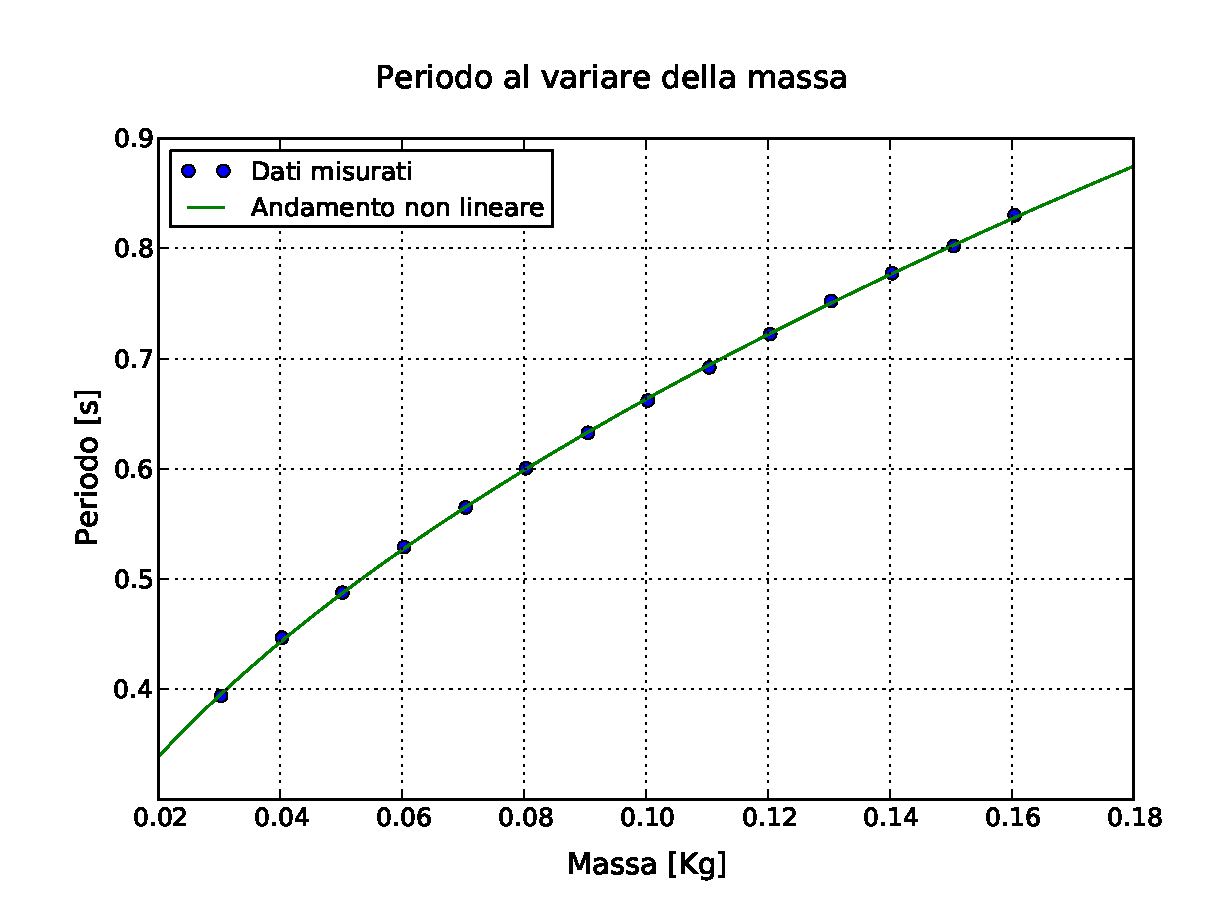
\includegraphics[width=120mm]{immagini/periodo_massa.pdf}
    \caption{Il grafico mostra il periodo di oscillazione della molla al variare della massa ad essa appesa.
        Le barre d'errore su massa e periodo non sono mostrate in quanto molto piccole e difficilmente leggibili.
        Come si vede chiaramente il periodo non dipende dalla massa in modo lineare, al contrario, segue una legge del tipo
        $\sqrt{a + bm}$, con coefficienti a e b, come quella tracciata in figura.}
    \label{fig:periodo_massa}
\end{SCfigure}

\begin{SCfigure}
    \centering
    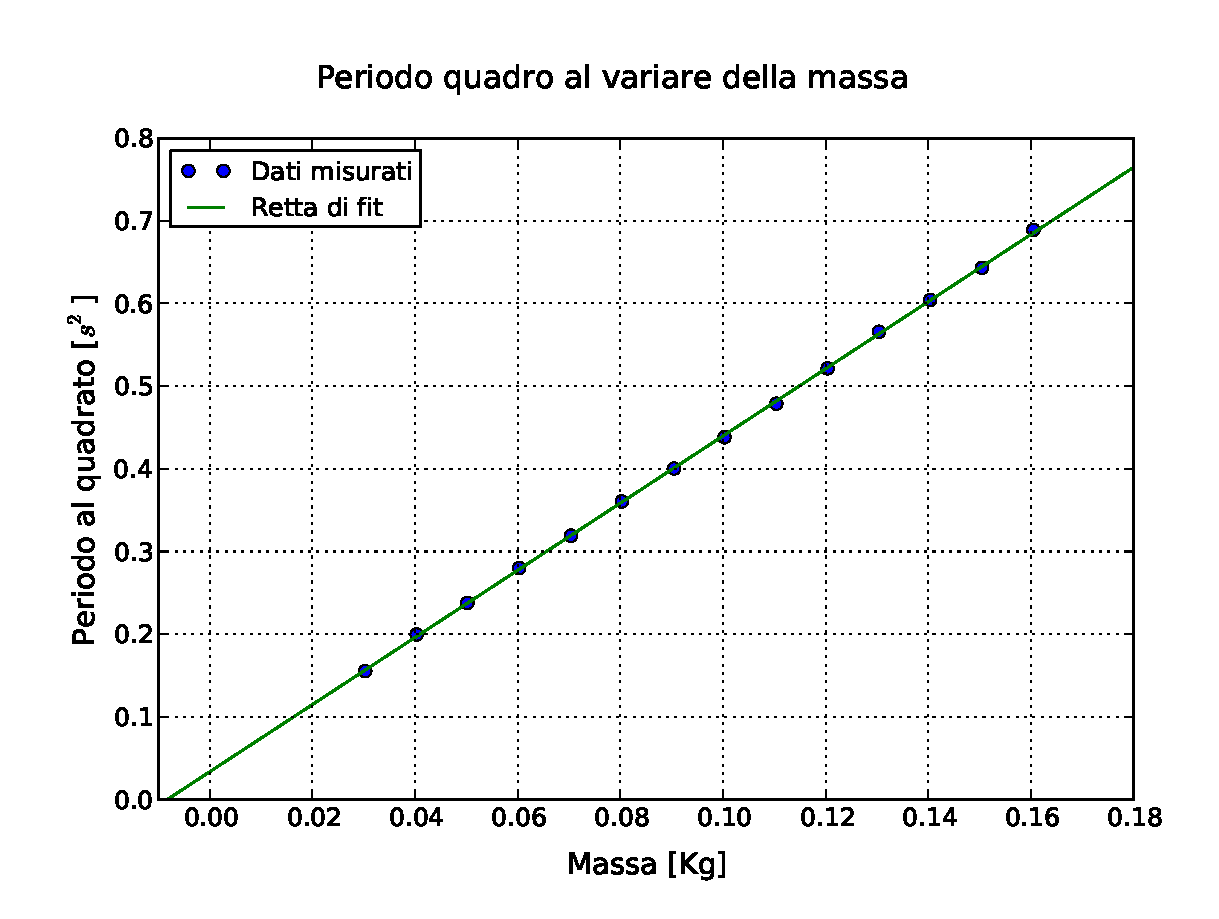
\includegraphics[width=120mm]{immagini/periodo2_massa.pdf}
    \caption{boh}
    \label{fig:periodo2_massa}
\end{SCfigure}

\subsubsection{Massa efficace della molla}

Il sistema molla più massa studiato è un sistema reale che non rispecchia con fedeltà assoluta la semplicistica
legge (\ref{eq:pp}) ricavata in precenza. Infatti, per ricavare la (\ref{eq:pp}) con analisi dimensionale
si devono fare delle ipotesi sulle grandezze che influenzano il periodo, e si può facilmente mancare di considerare qualche
fattore importante. Per esempio non sono state prese in considerazione le caratteristiche proprie della molla stessa
al di fuori della sua costante elastica. La molla possiede infatti una massa ed altre caratteristiche
come una dissipazione interna, che sono state trascurate. Il principale fattore che è stato trascurato
è l'inerzia (massa) della molla stessa. Questo effetto si può notare nel grafico in figura \ref{fig:periodo2_massa},
dove si vede che la retta che meglio interpreta i dati non passa per l'origine.

Questi effetti apparentemente complicati, possono essere semplificati introducendo un fattore correttivo $m_e$ detto
\emph{massa efficace} della molla, che ne tiene conto. Questo fattore correttivo va a modificare l'equazione (\ref{eq:pp}) che diventa

\begin{equation}
    \mathcal{T} \, = \, \mathcal{C} \, \sqrt{\frac{M}{k}}
    \label{eq:ppme}
\end{equation}
%
dove $M = m_e + m$. Quindi nella figura \ref{fig:periodo2_massa} la retta interseca l'asse delle ascissa
nel punto $m_e$.

La massa efficace non è la massa della molla stessa, ma la massa fittizia che occorrerebbe
appendere ad una molla ideale per rendere le sue oscillazioni identice a quelle della molla reale.

Troviamo ora la relazione che collega la massa efficace $m_e$ della molla alla sua massa reale $\mu$.
Immaginiamo di far oscillare la molla di massa $\mu$ e lunghezza $L$ mantenendo fisso un estremo.
Consideriamo un pezzetto infinitesimo della molla a distanza $\ell$ dall'estremo fisso. La massa del pezzo
varrà $\mu \, d\ell / L$. Ipotizzando che la velocità di tale pezzo sia proporzionale alla distanza dall'estremo
fisso, si ottiene che la sua velocità è $v \, \ell / L$, dove $v$ è la velocità dell'estremo libero.
Calcoliamo l'energia cinetica tramite l'integrale:

\begin{equation*}
    E_k \, = \, \int_0^L \frac{1}{2} \frac{\mu v^2}{L^3} \ell^2 \, d\ell \, = \,
    \frac{1}{2} \frac{\mu v^2}{L^3} \int_0^L \ell^2 \, d\ell = \frac{1}{6} \mu v^2
\end{equation*}
%
Tuttavia, per una massa ideale con le stesse oscillazioni, vale:

\begin{equation*}
    E_k \, = \, \frac{1}{2} m_e v^2
\end{equation*}
%
Eguagliando le due equazioni si ottiene $m_e = \mu/3$ ovvero $\mu = 3\,\,m_e$. 

\subsubsection{Calcolo dei parametri $\mathcal{C}$ e $m_e$ mediante il metodo della regressione lineare}
Considerando l'equazione (\ref{eq:ppme}) e analizzandola tenendo conto del nuovo valore della massa $M = m_e + m$, otteniamo:

\begin{equation*}
	\mathcal{T} \,=\, \mathcal{C} \, \sqrt{\frac{M}{k}}	\,\,\,=>\,\,\, \mathcal{T} \,=\, \mathcal{C} \, \sqrt{\frac{m_e + m}{k}}
\end{equation*}
%
pertanto elevando tutti i membri al quadrato otteniamo:

\begin{equation*}
	\mathcal{T}^2 \,=\, \mathcal{C}^2 \,\, \frac{(m_e + m)}{k}
\end{equation*}
%
Che si può riscrivere come segue:

\begin{equation}
	\mathcal{T}^2 \,\,=\,\, \frac{\mathcal{C}^2}{k} m_e \,+\, \frac{\mathcal{C}^2}{k} m
	\label{eq:mCspezzati}
\end{equation}
%
ed inoltre, la si può rendere più leggibile, scivendola nel seguente modo:

\begin{equation}
	y \,=\, A \,+\, Bx
	\label{eq:pppar}
\end{equation}
%
dove $x \equiv m$ (massa applicata) $y \equiv \mathcal{T}^2$, $A \equiv \frac{\mathcal{C}^2}{k} \, m_e$ e $B \equiv \frac{\mathcal{C}^2}{k}$.\\
Vogliamo quindi determinare i valori di A e B che minimizzano la discrepanza mediante la tecnica della regressione lineare pertanto procediamo con il metodo utilizzato anche nella sezione due.
\begin{itemize}
\item{calcoliamo la discrepanza:
		\begin{equation*}
			\text{discrepanza} \,=\, \sum_{i=1}^{13} \frac{(y_i - A - Bx_i)^2}{(\delta y_i)^2}
		\end{equation*}
		%
		ricordando che l'incertezza sull'asse delle ascisse è la stessa incertezza sulla massa ovvero $\delta m_i$ che in questa analisi poniamo uguli a $\delta x_i$.}
\item{Prima di procedere con l'analisi è necessario verificare che l'incertezza relativa alle masse sia trascurabile rispetto a quella dei periodi al quadrato. Per accertarlo è stato necessario fare una stima preliminare del parametro B. Dal momento che dal grafico è impossibile individuare le rette di massima e minima pendenza abbiamo deciso di ricavare il parmetro B valutando il coefficiente angolare della retta utilizzando il classico rapporto tra due punti del grafico, ovvero:

	\begin{equation*}
		\text{B} \,\,=\,\, \frac{\mathcal{T}_{14} - \mathcal{T}_{1}}{m_{14} - m_1} \,\,=\,\, 4.09 \,\, s^2 \,\,\,[verificare \,\,\,cifre]
	\end{equation*}
	%
	quindi grazie a questo valore di B siamo in grado di stimare l'incertezza trasferita, ovvero: $\sigma m_{tras} \,\,=\,\, B \, \sigma m$ dove $\sigma m$ rappresenta l'errore tipo di misura sulla massa. Abbiamo notato che questo valore è 10 volte minore rispetto all'incertezza sul periodo quadrato, e quindi poichè l'incertezza totale risulta essere la seguente
	
	\begin{equation*}
		\delta y_i \,=\, \sqrt{(\delta \mathcal{T}_k^2)^2 + \sigma m_{tras}^2} 
	\end{equation*}	
	%
	possiamo notare che sotto radice il termine $\sigma m_{tras}^2$ risulta essere 100 volte minore di $(\delta \mathcal{T}_k^2)^2$ quindi lo si può considerare trascurabile rispetto all'incertezza rispetto al periodo quadro.
	}
\item{quindi per quanto studiato in classe abbiamo che:

		\begin{equation*}
			A \,=\, \frac{(\sum_i w_i x_i^2)(\sum_i w-i y_i) - (\sum_i w_i x_i)(\sum_i w_i x_i y_i)}{\Delta} \,=\, 0.033655 \,\, s^2
		\end{equation*}
		%
		\begin{equation*}
			B \,=\, \frac{(\sum_i w_i)(\sum_i w-i x_i y_i) - (\sum_i w_i y_i)(\sum_i w_i x_i)}{\Delta} \,=\, 4.0603 \,\, s^2 / kg
		\end{equation*}
		%
		dove:
		\begin{equation*}
			\Delta \,=\, (\sum_i w_i)(\sum_i w_i x_i^2) - (\sum_i w_i x_i)^2 \,\,\,\,\,\,\, e \,\,\,\,\,\,\,
			w_i \,=\, \frac{1}{(\delta y_i)^2}
		\end{equation*}}
\item{di conseguenza abbiamo che le incertezze relative su A e B sono:

		\begin{equation*}
			(\delta A)^2 \,=\, \frac{\sum_i w_i x_i^2}{\Delta}  \,\,\,\,\, e \,\,\,\,\,
			(\delta B)^2 \,=\, \frac{\sum_i w_i}{\Delta} 
		\end{equation*}}
\end{itemize} 
Quindi possiamo riassumere i risultati di questa procedura in questo modo:

\begin{equation*}
	A \,\pm\, \delta A \,=\, (0.034 \,\, \pm \,\, 0.001) \,\,s^2 \,\,\,\,\, e \,\,\,\,\,
	B \,\pm\, \delta B \,=\, (4.06 \,\, \pm \,\, 0.01) \,\,s^2 \,/\, kg
\end{equation*}
%
Perciò noti questi parametri possiamo risalire ai valoti di $\mathcal{C}$ e $m_e$ risolvendo l'equazione in (\ref{eq:pppar}) e utilizzando come valore di k quello trovato nell'analisi dati della sezine precedente ovvero $K_0 \,=\, 9.64 \, N/m$ otteniamo quanto segue:

\begin{equation*}
	\mathcal{C} \,\pm\, \delta \mathcal{C} \,\,=\,\, (6.256 \, \pm \, 0.007)
\end{equation*}
%
\begin{equation*}
	m_e \, \pm \, \delta m_e \,\,=\,\, (0.0083 \,\, \pm \,\, 0.0002) \,\, kg
\end{equation*}

\subsubsection{Test del chi quadro}
Procediamo ora a verificare che le equazioni (\ref{eq:mCspezzati}) e (\ref{eq:pppar}) i valori sopra ottenuti siano compatibili con i dati sperimentali mediante il test del chi quaro. Ricordiamo che il numero di gradi di libertà in questo caso non è più N - 1, ma risulta essere N - 2 in qunto due dati sono stati utilizzati per calcolare i  valori sperimentali A e B. Pertanto ci aspettiamo che:

\begin{equation*}
	\chi_{oss}^2 \,=\, \sum_{i=1}^{N} \frac{(y_i - A - Bx_i)^2}{(\delta y_i)^2} \,\simeq\, N - 2 \quad \text{ricordando che} \quad \chi_{teo}^2 \,\,:=\,\, N - 2
\end{equation*}
%
il nostro valore del chi quadro osservato è:

\begin{equation*}
	\chi_{oss}^2 \,\,=\,\, 21.1 \quad \text{che risulta essere compatibile con il} \quad \chi_{teo}^2
\end{equation*}
%
in quanto $\chi_{teo}^2 \, \pm \, \delta \chi_{teo}^2 \,\,=\,\, 12.0 \, \pm \, 4.9$ pertanto la differenza tra i due chi quadro risulta essere la seguente:

\begin{equation*}
	|R| \,\,=\,\, (\chi_{oss}^2 - \chi_{teo}^2) \,\,=\,\, 9.1
\end{equation*}
%
mentre, posto a priori un fattore di copertura k = 2, l'errore sul resto è:

\begin{equation*}
	k \, \sigma_{R} \,\,=\,\, 9.8
\end{equation*}
%
e quindi risulta che $|R| \, \leq \, k \, \sigma_{R}$.\\

Dal momento che il chi quadro osservato pur essendo compatibile con la predizione teorica risulta essere molto maggiore del chi quadro teorico abbiamo deciso di rifare il fit per ottenere una migliore stima deglle inceretezze sul periodo che probabilmente sono state sottostimate.\\
Pertanto rifacendo la procedura del fit vogliamo aggiustare il valore delle incertezze in modo da eguagiare i due chi, ovvero quello teorico e sperimentale. Pertanto:

RIGUARDAREEEEEEEEEE

\begin{equation*}
	\chi_{oss}^2 \,=\, \sum_{i=1}^{N} \frac{(y_i - A - Bx_i)^2}{(\delta y_i)^2} \,=\, \chi_{teo}^2 
\end{equation*}
%
e così facendo troviamo un coefficiente che moltiplicato per il precedente $\delta y_i$ ci restituisce una nuova varianza grazie alla quale i due chi risulteranno uguali. Infatti abbiamo ottenuto:
	
\begin{equation*}
	\chi_{oss}^2 \,\,=\,\, \frac{1}{\delta y_{i}^2} \sum_{1}^{N} (y_i - A - Bx_i)^2  \,\,=\,\, \chi_{teo}^2
\end{equation*}
%
poichè sappiamo che:
	
\begin{equation*}
	\chi_{teo}^2 \,=\, \nu \quad \quad con \quad \quad
	\nu \,=\, N - 1 \quad \quad e \quad \quad
	\delta x_{posteriori}^2 \,\,=\,\, \frac{\chi_{oss}^2}{\nu} \, \delta x_{priori}^2
\end{equation*}
%
con $\nu$ che rappresenta i gradi di libertà.
Quindi si ottiene che:

\begin{equation*}
	\delta x_{posteriori} \,=\,  \,m \,\,=\,  \,\, mm
\end{equation*}	 
 





